\begin{frame}
\frametitle{B+ деревья}
\begin{itemize}
  \item B+ дерево - идеально сбалансированное сильно ветвистое дерево
  поиска, которое хранит значения только в листьях:
  \begin{itemize}
    \item растояние от корня до всех листьев одинаковое;
    \item каждый узел кроме корня хранит не менее B ключей, где B
    некоторый фиксированный параметр дерева;
    \item словарь хранит пары - (ключ, значение) - все внутренние узлы
    хранят только ключи, и только листья хранят полные пары.
  \end{itemize}
\end{itemize}
\end{frame}

\begin{frame}
\frametitle{Инварианты B+ деревьев}
\begin{itemize}
  \item Каждый узел кроме корня хранит от $B$ до $2B$ ключей (ссылок на
  дочерние узлы):
  \begin{itemize}
    \item соответсвенно высота дерева растет как $log_B$.
  \end{itemize}
  \item Корень, если он не является листом соедржит как минимум 2 ключа:
  \begin{itemize}
    \item это условие определяет когда можно удалить текущий корень и уменьшить 
    высоту дерева.
  \end{itemize}
\end{itemize}
\end{frame}

\begin{frame}
\frametitle{Балансировка B+ деревьев}
\begin{itemize}
  \item Бинарные деревья поиска, зачастую, используют повтороты:
  \begin{itemize}
    \item B деревья не используют повортов - их способ гораздо "топорнее".
  \end{itemize}
  \item Если в узле мало ключей:
  \begin{itemize}
    \item можно забрать часть ключей у соседа, если у него есть лишние;
    \item можно просто объединиться с соседом и продолжить балансировку
    рекурсивно от родителя;
    \item если соседей нет - значит мы корень.
  \end{itemize}
  \item Если в узле много ключей:
  \begin{itemize}
    \item просто разбиваем узел на два и продолжаем балансировку рекурсивно от
    родителя.
  \end{itemize}
\end{itemize}
\end{frame}

\begin{frame}
\frametitle{Пример вставки в B+ дерево}
\begin{center}
  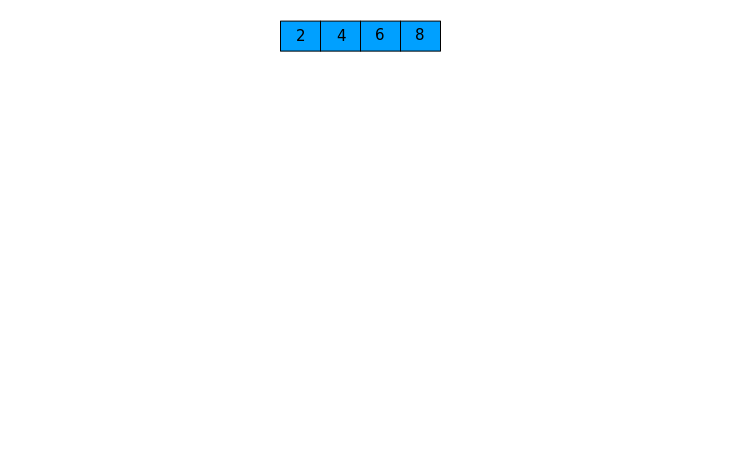
\includegraphics[width=.8\linewidth]{btree0.png}
\end{center}
\end{frame}

\begin{frame}
\frametitle{Пример вставки в B+ дерево}
\begin{center}
  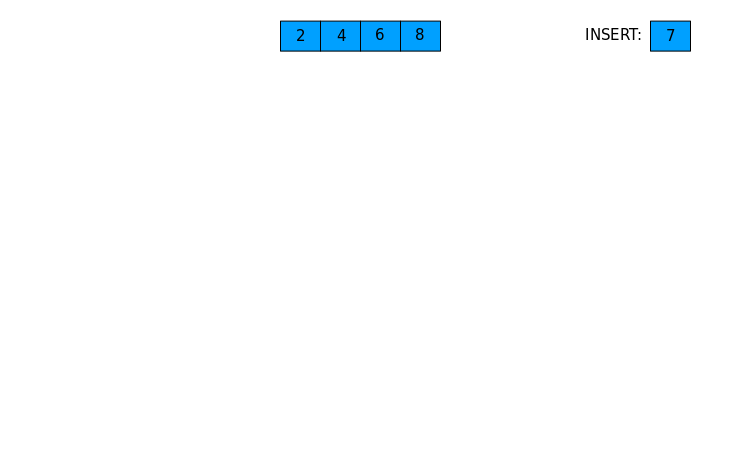
\includegraphics[width=.8\linewidth]{btree1.png}
\end{center}
\end{frame}

\begin{frame}
\frametitle{Пример вставки в B+ дерево}
\begin{center}
  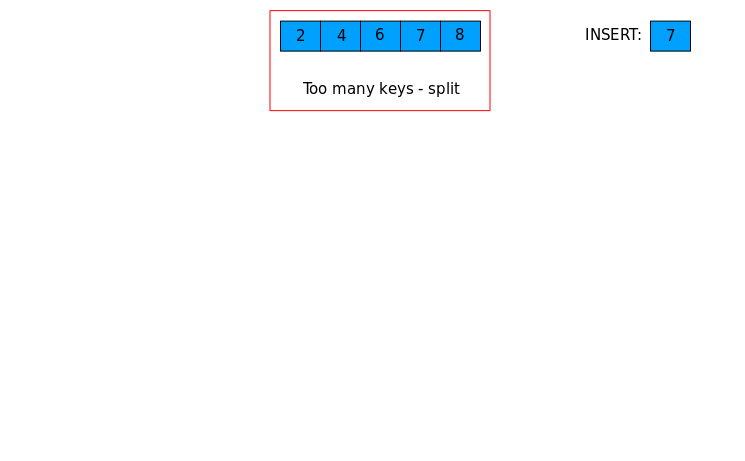
\includegraphics[width=.8\linewidth]{btree2.png}
\end{center}
\end{frame}

\begin{frame}
\frametitle{Пример вставки в B+ дерево}
\begin{center}
  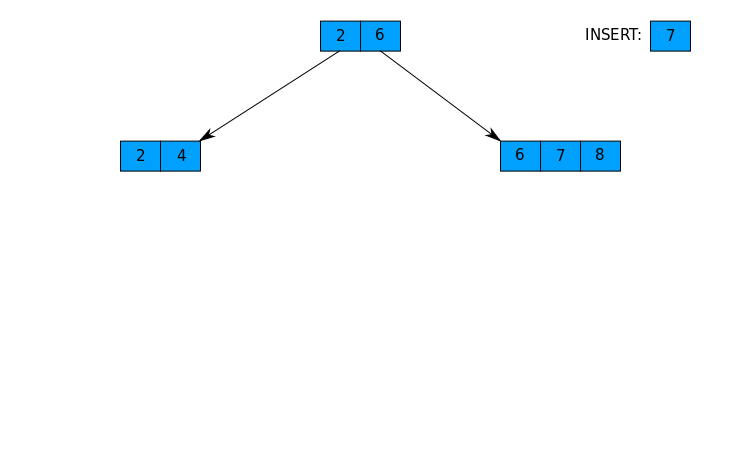
\includegraphics[width=.8\linewidth]{btree3.png}
\end{center}
\end{frame}

\begin{frame}
\frametitle{Пример вставки в B+ дерево}
\begin{center}
  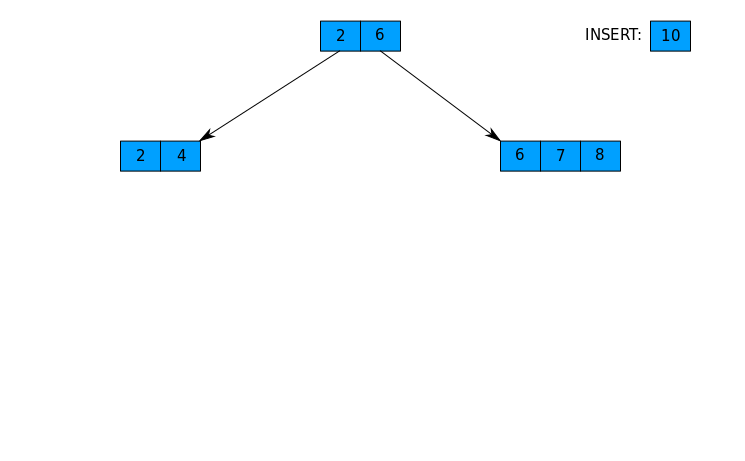
\includegraphics[width=.8\linewidth]{btree4.png}
\end{center}
\end{frame}

\begin{frame}
\frametitle{Пример вставки в B+ дерево}
\begin{center}
  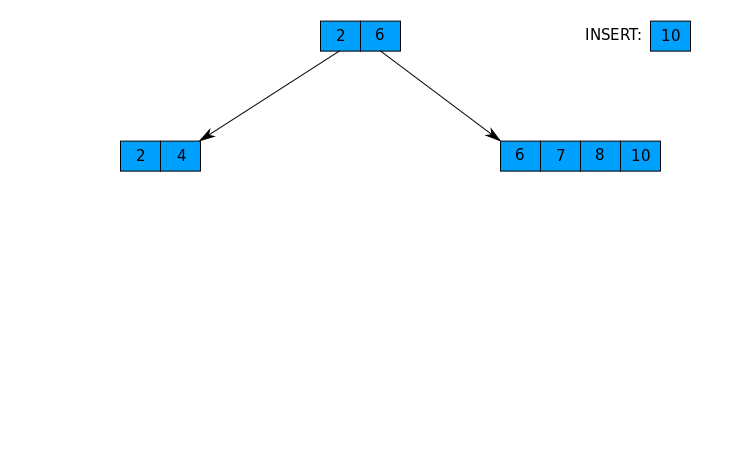
\includegraphics[width=.8\linewidth]{btree5.png}
\end{center}
\end{frame}

\begin{frame}
\frametitle{Пример вставки в B+ дерево}
\begin{center}
  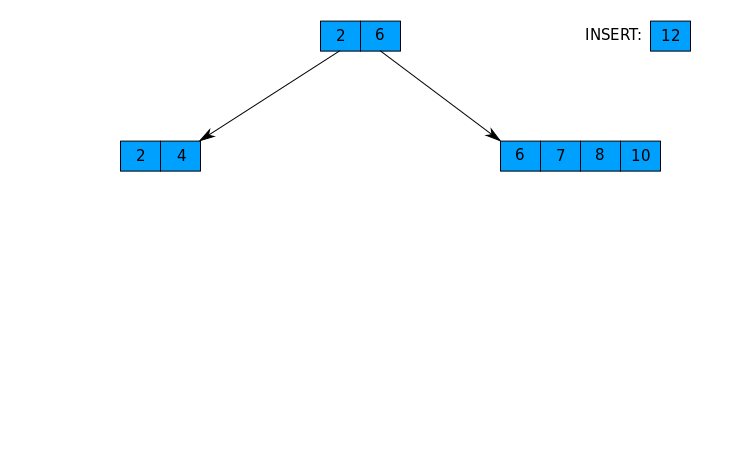
\includegraphics[width=.8\linewidth]{btree6.png}
\end{center}
\end{frame}

\begin{frame}
\frametitle{Пример вставки в B+ дерево}
\begin{center}
  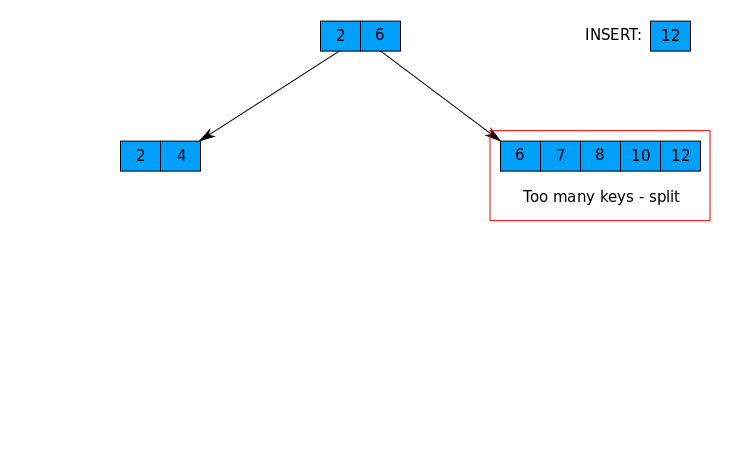
\includegraphics[width=.8\linewidth]{btree7.png}
\end{center}
\end{frame}

\begin{frame}
\frametitle{Пример вставки в B+ дерево}
\begin{center}
  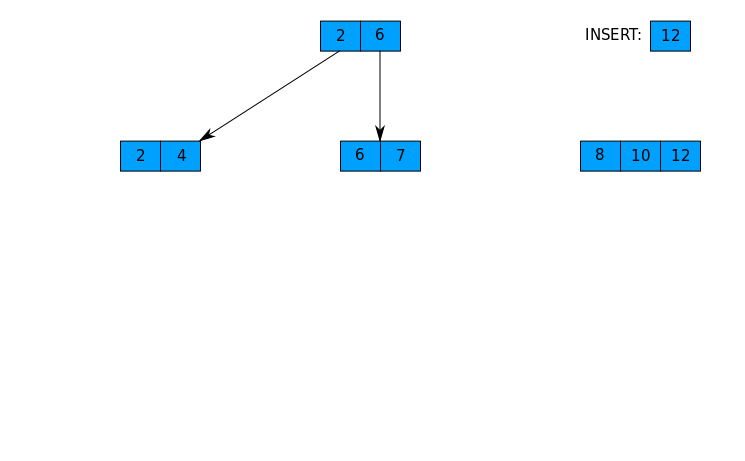
\includegraphics[width=.8\linewidth]{btree8.png}
\end{center}
\end{frame}

\begin{frame}
\frametitle{Пример вставки в B+ дерево}
\begin{center}
  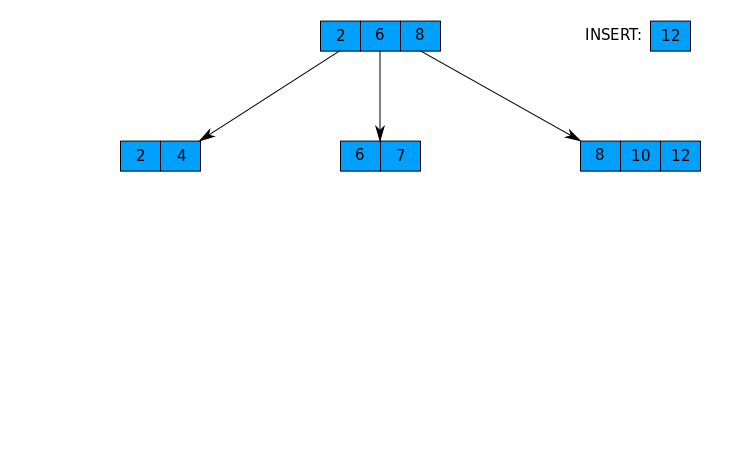
\includegraphics[width=.8\linewidth]{btree9.png}
\end{center}
\end{frame}

\begin{frame}
\frametitle{Пример вставки в B+ дерево}
\begin{center}
  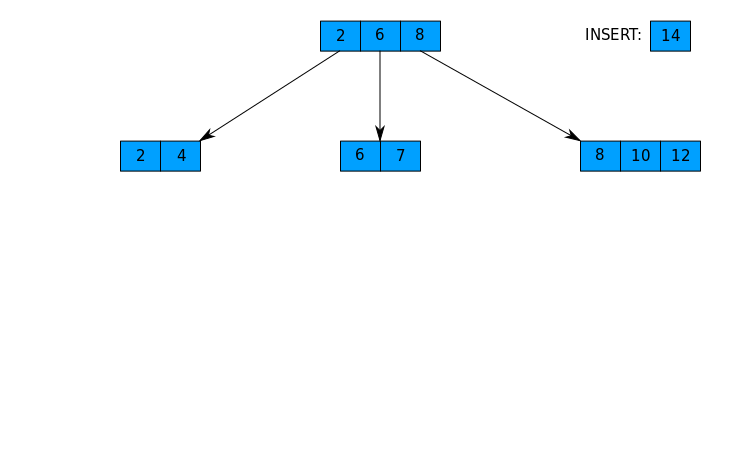
\includegraphics[width=.8\linewidth]{btree10.png}
\end{center}
\end{frame}

\begin{frame}
\frametitle{Пример вставки в B+ дерево}
\begin{center}
  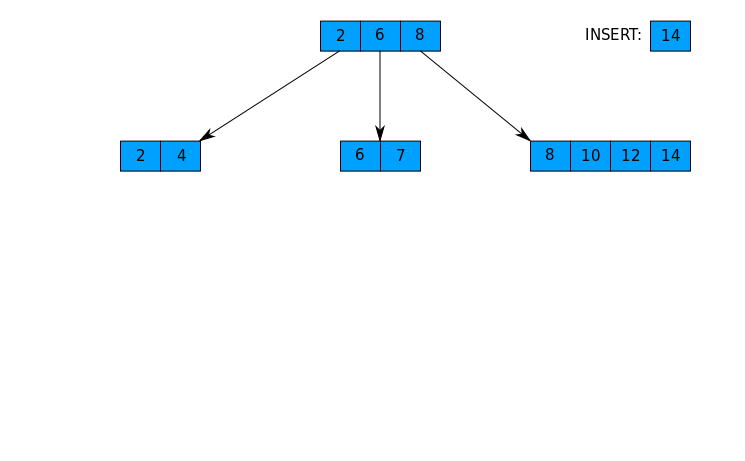
\includegraphics[width=.8\linewidth]{btree11.png}
\end{center}
\end{frame}

\begin{frame}
\frametitle{Пример вставки в B+ дерево}
\begin{center}
  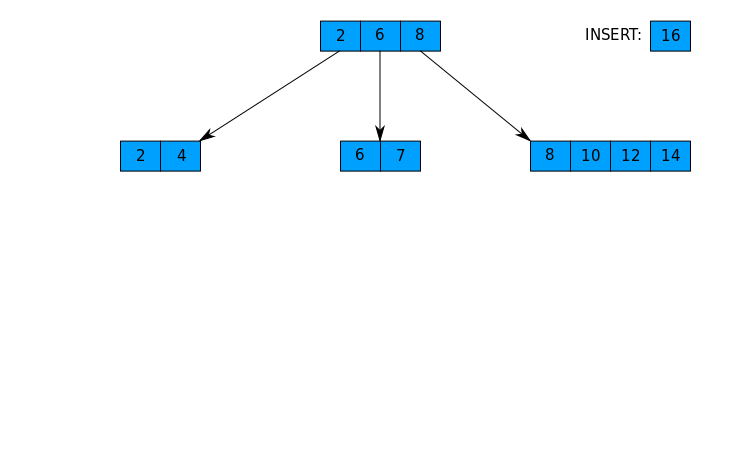
\includegraphics[width=.8\linewidth]{btree12.png}
\end{center}
\end{frame}

\begin{frame}
\frametitle{Пример вставки в B+ дерево}
\begin{center}
  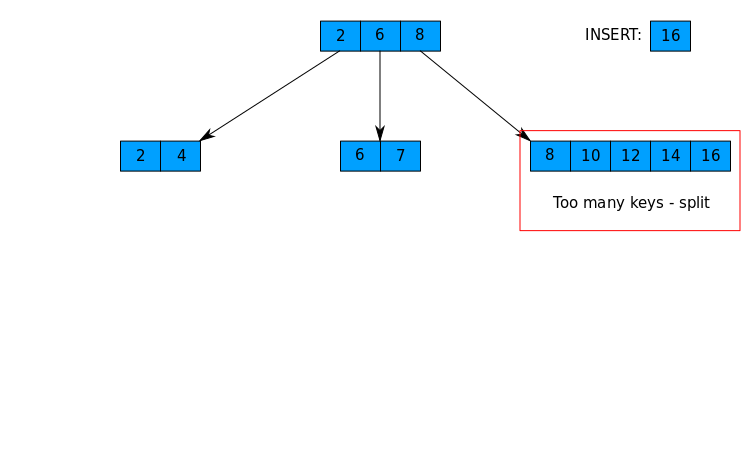
\includegraphics[width=.8\linewidth]{btree13.png}
\end{center}
\end{frame}

\begin{frame}
\frametitle{Пример вставки в B+ дерево}
\begin{center}
  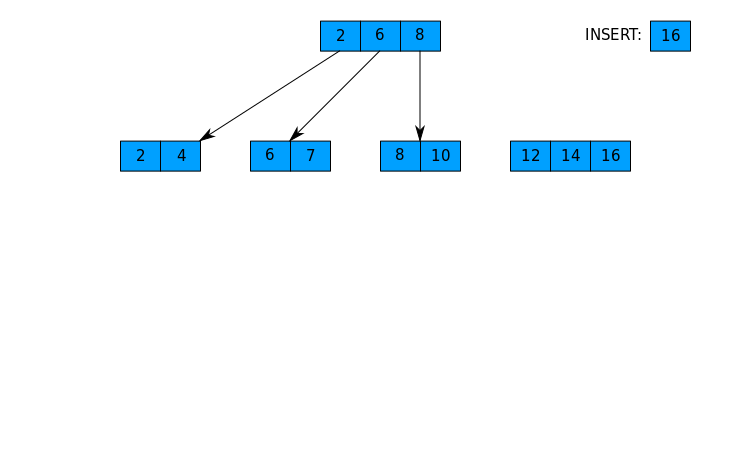
\includegraphics[width=.8\linewidth]{btree14.png}
\end{center}
\end{frame}

\begin{frame}
\frametitle{Пример вставки в B+ дерево}
\begin{center}
  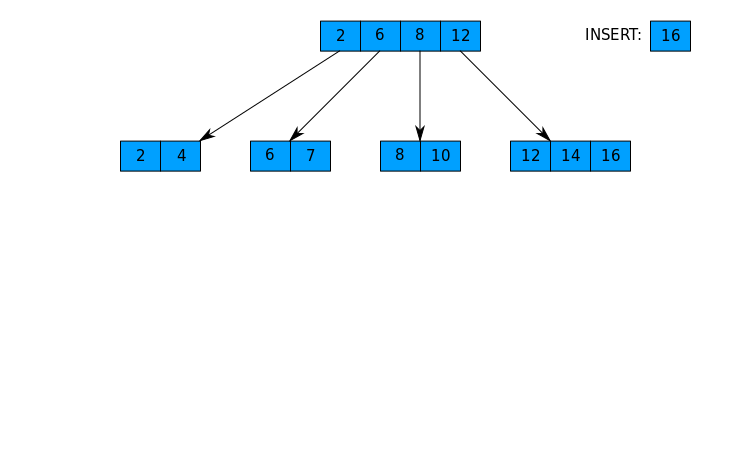
\includegraphics[width=.8\linewidth]{btree15.png}
\end{center}
\end{frame}

\begin{frame}
\frametitle{Пример вставки в B+ дерево}
\begin{center}
  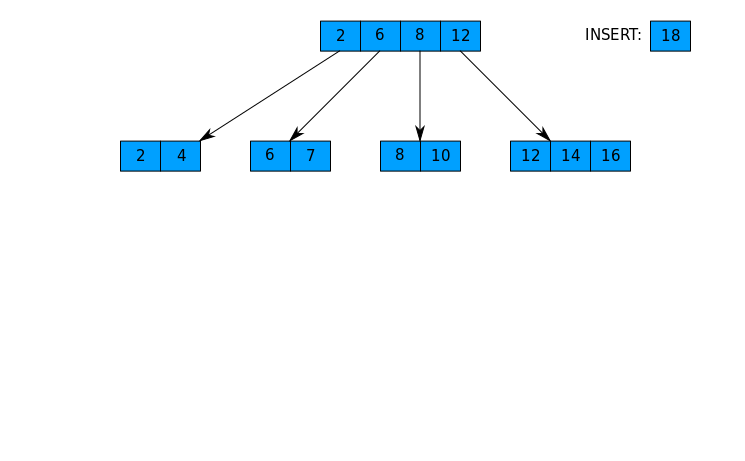
\includegraphics[width=.8\linewidth]{btree16.png}
\end{center}
\end{frame}

\begin{frame}
\frametitle{Пример вставки в B+ дерево}
\begin{center}
  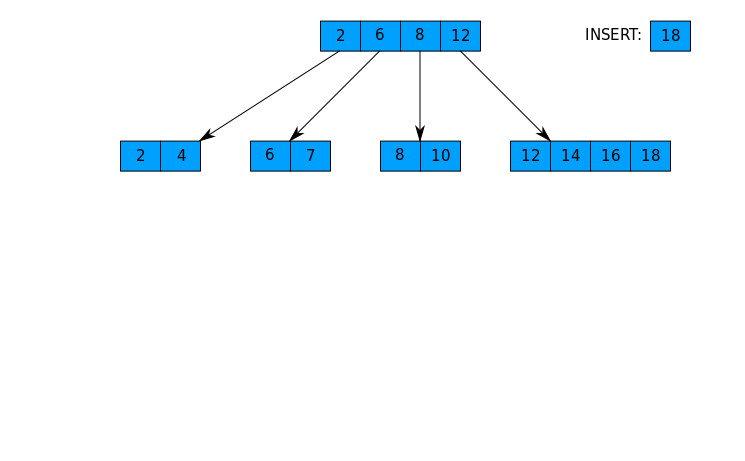
\includegraphics[width=.8\linewidth]{btree17.png}
\end{center}
\end{frame}

\begin{frame}
\frametitle{Пример вставки в B+ дерево}
\begin{center}
  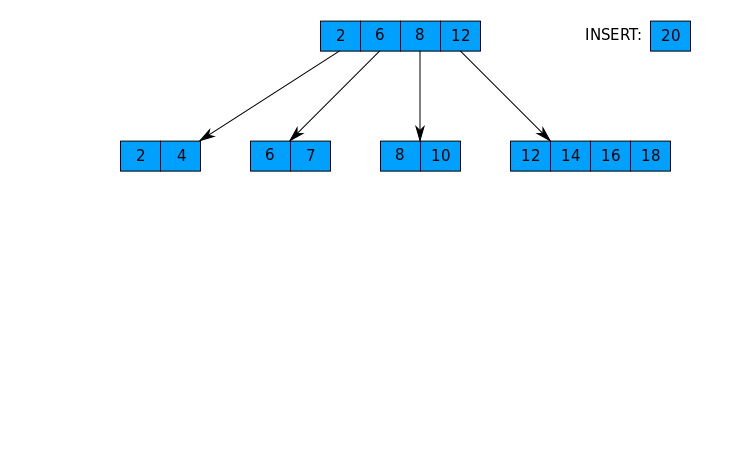
\includegraphics[width=.8\linewidth]{btree18.png}
\end{center}
\end{frame}

\begin{frame}
\frametitle{Пример вставки в B+ дерево}
\begin{center}
  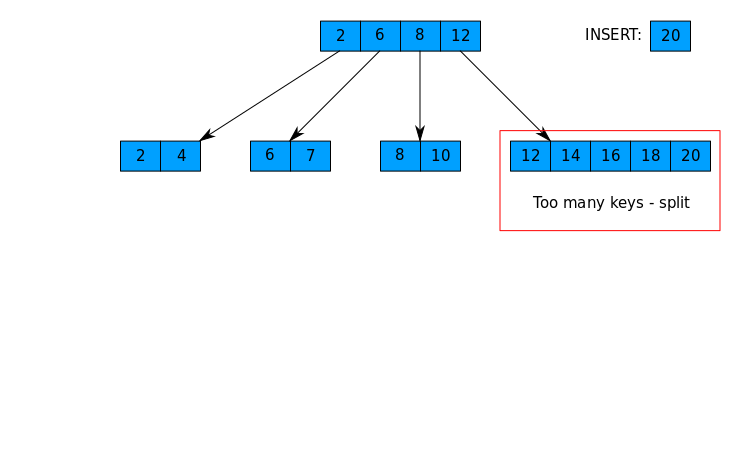
\includegraphics[width=.8\linewidth]{btree19.png}
\end{center}
\end{frame}

\begin{frame}
\frametitle{Пример вставки в B+ дерево}
\begin{center}
  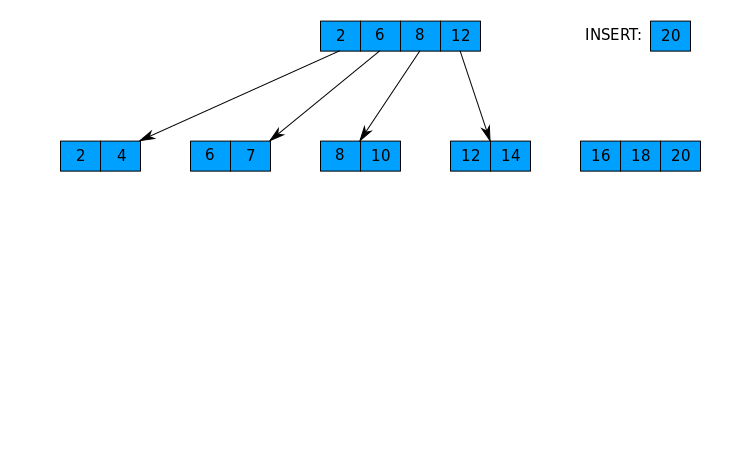
\includegraphics[width=.8\linewidth]{btree20.png}
\end{center}
\end{frame}

\begin{frame}
\frametitle{Пример вставки в B+ дерево}
\begin{center}
  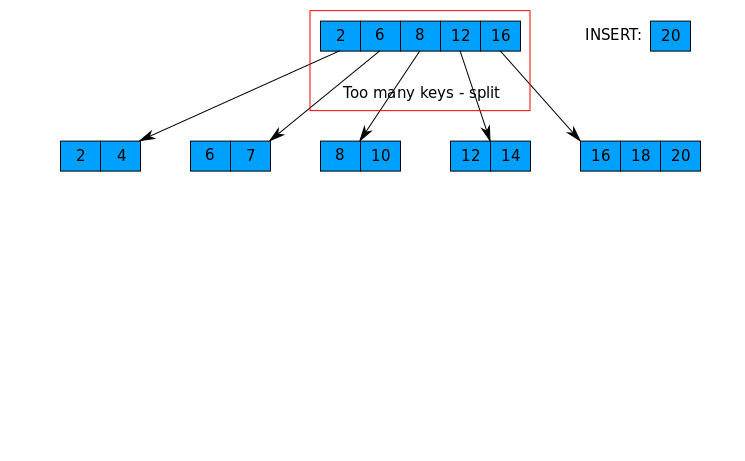
\includegraphics[width=.8\linewidth]{btree21.png}
\end{center}
\end{frame}

\begin{frame}
\frametitle{Пример вставки в B+ дерево}
\begin{center}
  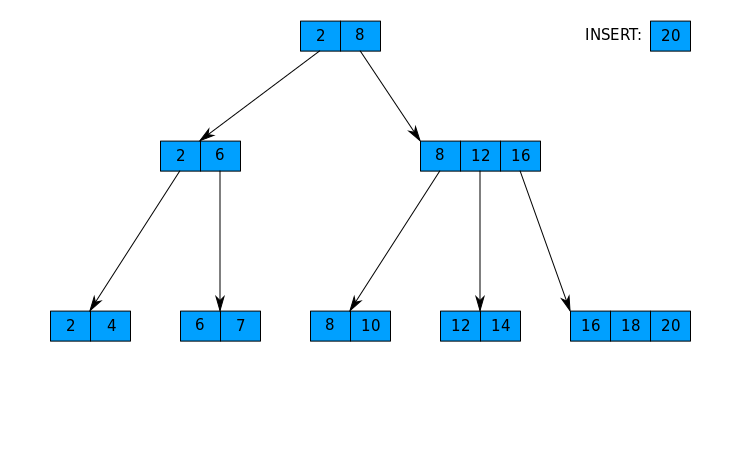
\includegraphics[width=.8\linewidth]{btree22.png}
\end{center}
\end{frame}

\begin{frame}
\frametitle{Пример вставки в B+ дерево}
\begin{center}
  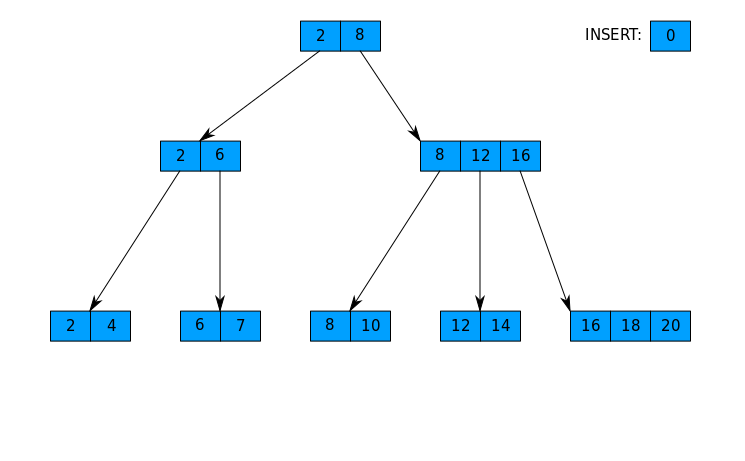
\includegraphics[width=.8\linewidth]{btree23.png}
\end{center}
\end{frame}

\begin{frame}
\frametitle{Пример вставки в B+ дерево}
\begin{center}
  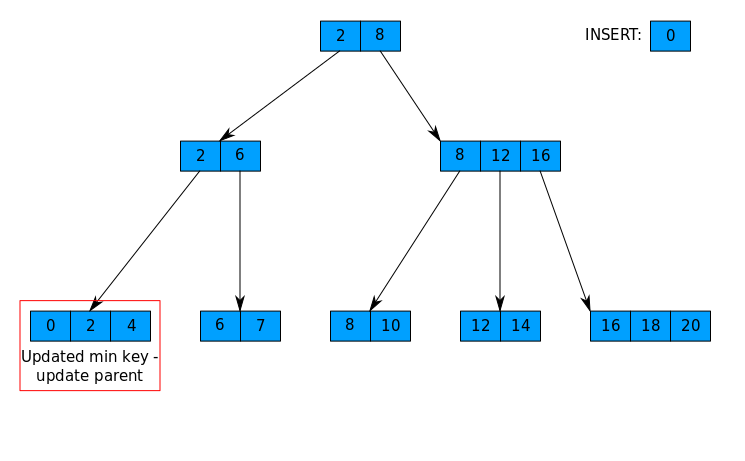
\includegraphics[width=.8\linewidth]{btree24.png}
\end{center}
\end{frame}

\begin{frame}
\frametitle{Пример вставки в B+ дерево}
\begin{center}
  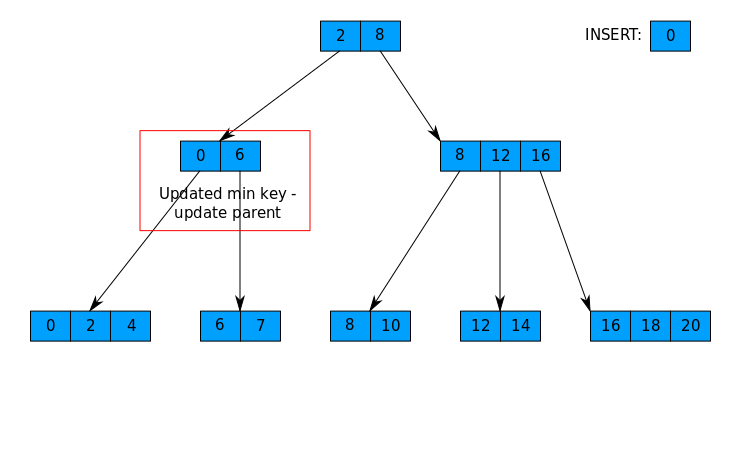
\includegraphics[width=.8\linewidth]{btree25.png}
\end{center}
\end{frame}

\begin{frame}
\frametitle{Пример вставки в B+ дерево}
\begin{center}
  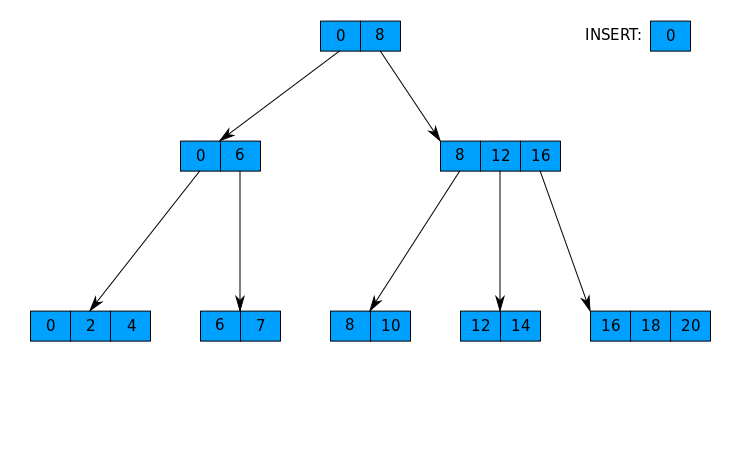
\includegraphics[width=.8\linewidth]{btree26.png}
\end{center}
\end{frame}

\begin{frame}
\frametitle{Пример удаления из B+ дерево}
\begin{center}
  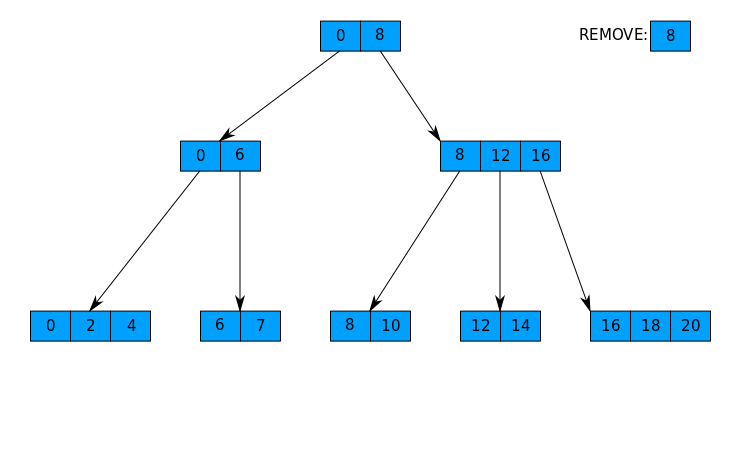
\includegraphics[width=.8\linewidth]{btree27.png}
\end{center}
\end{frame}

\begin{frame}
\frametitle{Пример удаления из B+ дерево}
\begin{center}
  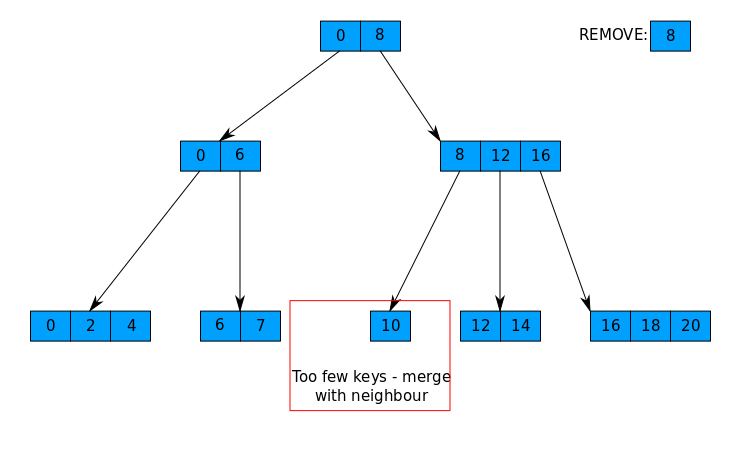
\includegraphics[width=.8\linewidth]{btree28.png}
\end{center}
\end{frame}

\begin{frame}
\frametitle{Пример удаления из B+ дерево}
\begin{center}
  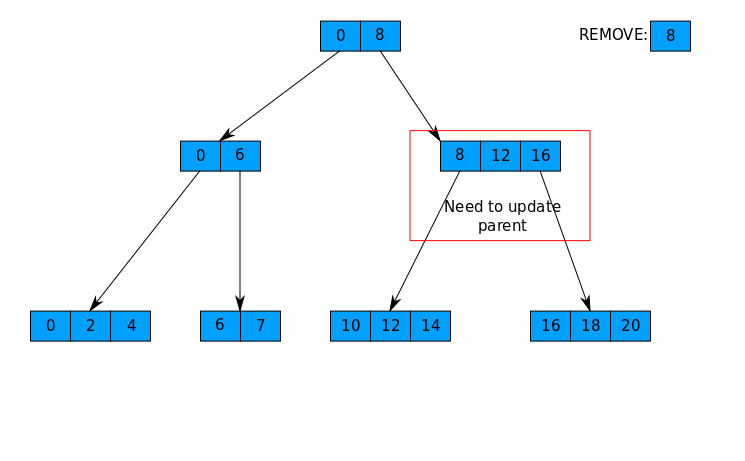
\includegraphics[width=.8\linewidth]{btree29.png}
\end{center}
\end{frame}

\begin{frame}
\frametitle{Пример удаления из B+ дерево}
\begin{center}
  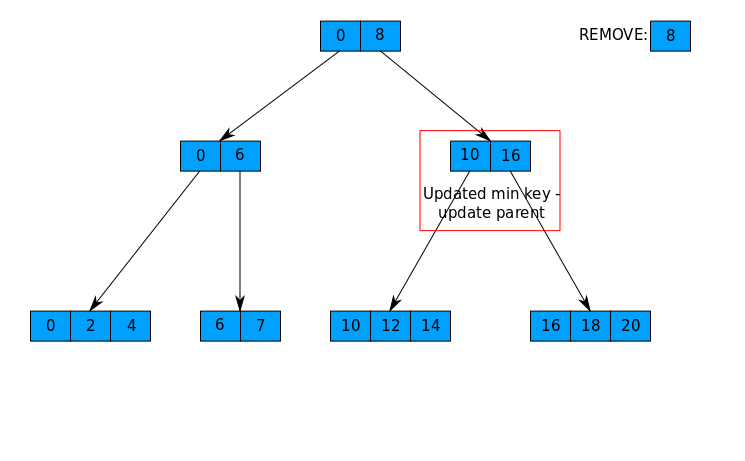
\includegraphics[width=.8\linewidth]{btree30.png}
\end{center}
\end{frame}

\begin{frame}
\frametitle{Пример удаления из B+ дерево}
\begin{center}
  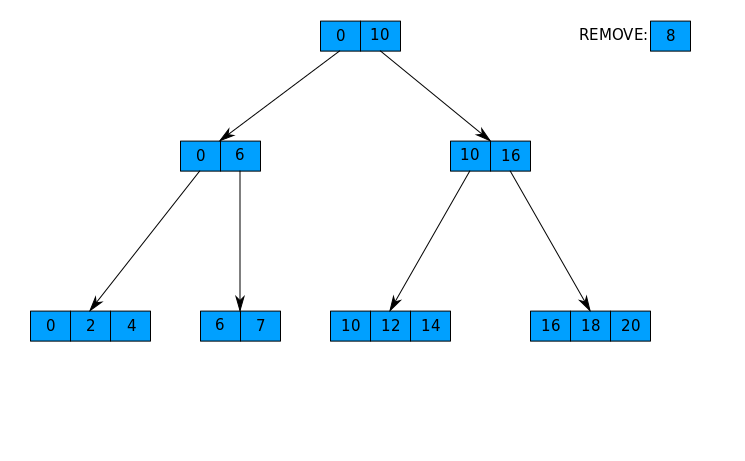
\includegraphics[width=.8\linewidth]{btree31.png}
\end{center}
\end{frame}

\begin{frame}
\frametitle{Пример удаления из B+ дерево}
\begin{center}
  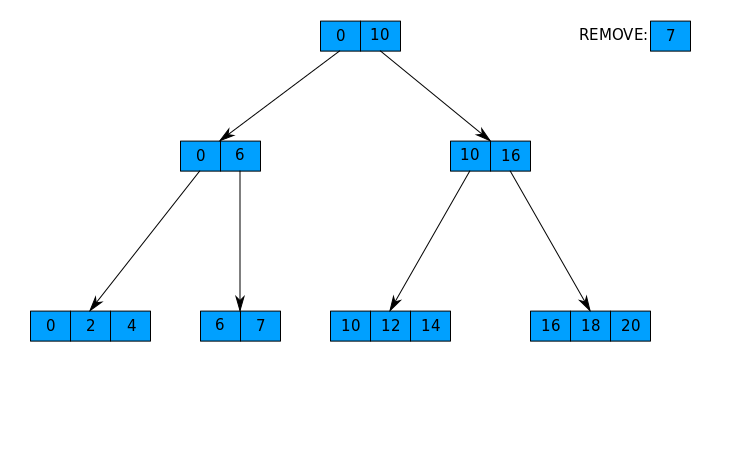
\includegraphics[width=.8\linewidth]{btree32.png}
\end{center}
\end{frame}

\begin{frame}
\frametitle{Пример удаления из B+ дерево}
\begin{center}
  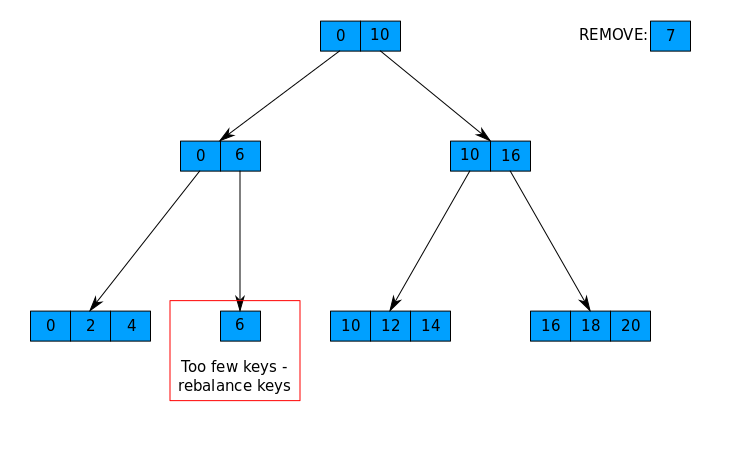
\includegraphics[width=.8\linewidth]{btree33.png}
\end{center}
\end{frame}

\begin{frame}
\frametitle{Пример удаления из B+ дерево}
\begin{center}
  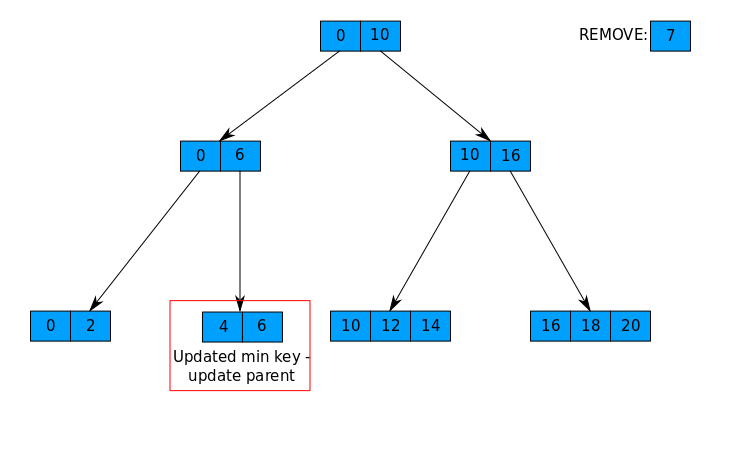
\includegraphics[width=.8\linewidth]{btree34.png}
\end{center}
\end{frame}

\begin{frame}
\frametitle{Пример удаления из B+ дерево}
\begin{center}
  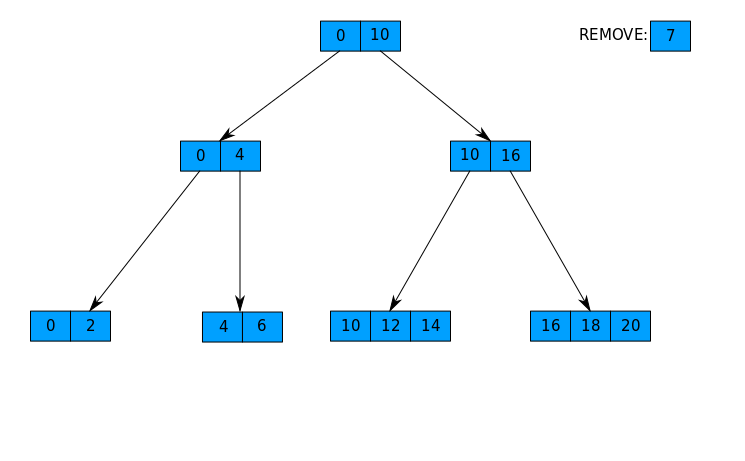
\includegraphics[width=.8\linewidth]{btree35.png}
\end{center}
\end{frame}

\begin{frame}
\frametitle{Пример удаления из B+ дерево}
\begin{center}
  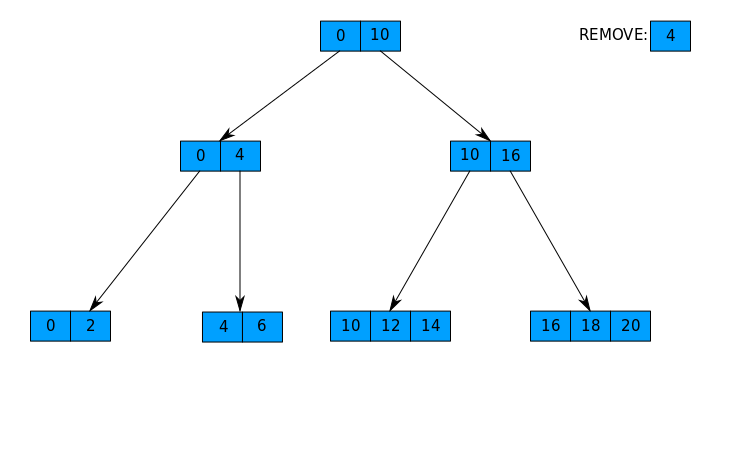
\includegraphics[width=.8\linewidth]{btree36.png}
\end{center}
\end{frame}

\begin{frame}
\frametitle{Пример удаления из B+ дерево}
\begin{center}
  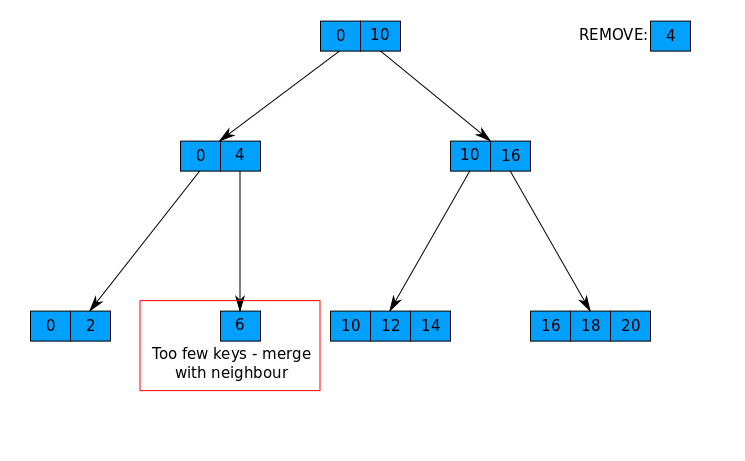
\includegraphics[width=.8\linewidth]{btree37.png}
\end{center}
\end{frame}

\begin{frame}
\frametitle{Пример удаления из B+ дерево}
\begin{center}
  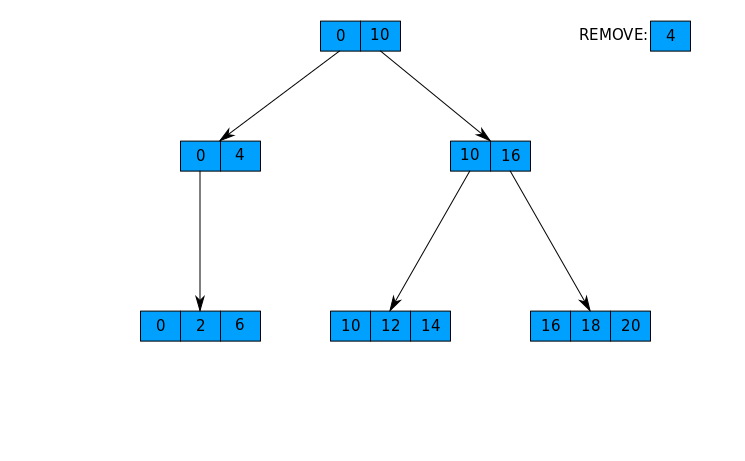
\includegraphics[width=.8\linewidth]{btree38.png}
\end{center}
\end{frame}

\begin{frame}
\frametitle{Пример удаления из B+ дерево}
\begin{center}
  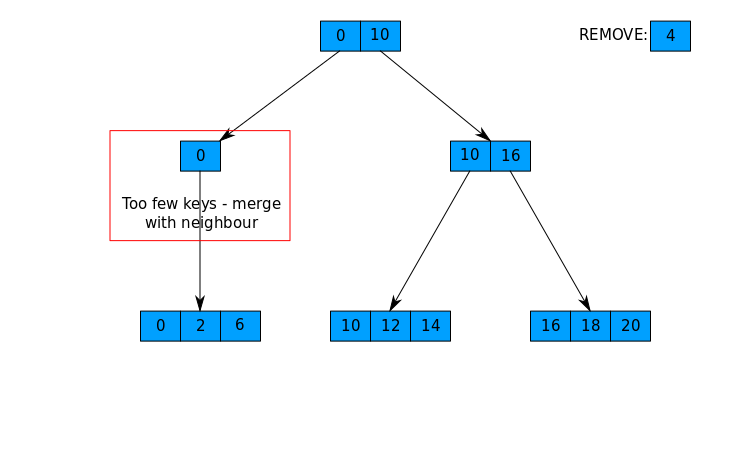
\includegraphics[width=.8\linewidth]{btree39.png}
\end{center}
\end{frame}

\begin{frame}
\frametitle{Пример удаления из B+ дерево}
\begin{center}
  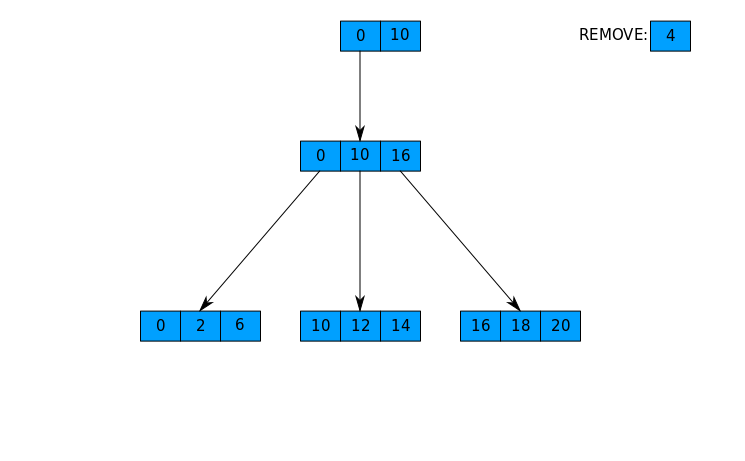
\includegraphics[width=.8\linewidth]{btree40.png}
\end{center}
\end{frame}

\begin{frame}
\frametitle{Пример удаления из B+ дерево}
\begin{center}
  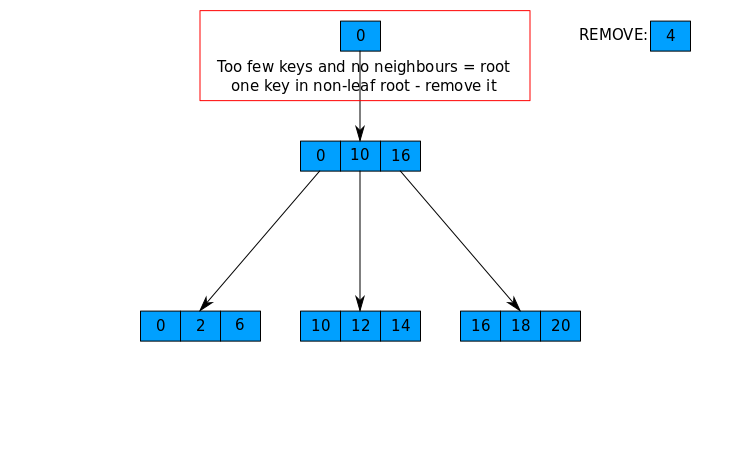
\includegraphics[width=.8\linewidth]{btree41.png}
\end{center}
\end{frame}

\begin{frame}
\frametitle{Пример удаления из B+ дерево}
\begin{center}
  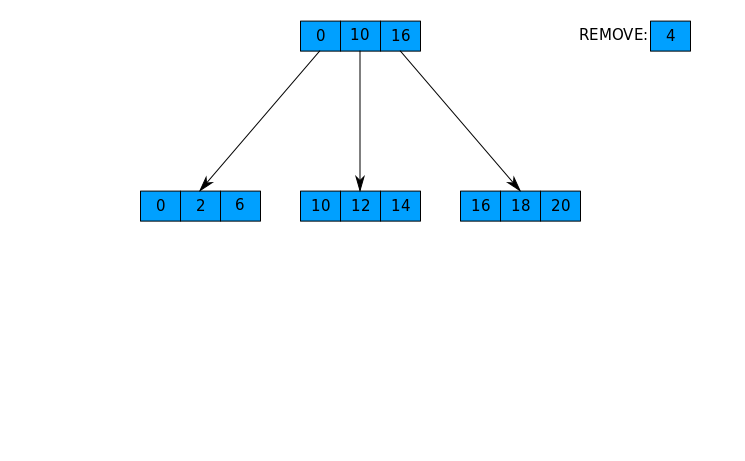
\includegraphics[width=.8\linewidth]{btree42.png}
\end{center}
\end{frame}
